%!TEX root = monsterhunter.tex
%!TEX encoding = UTF-8 Unicode

\newcommand*{\SBSep}{%
  \noindent
\includegraphics[height=5pt,width=\linewidth]{assets/stat-block-separator}\par
}

\renewcommand*{\hbPartCover}{assets/ext/lagiacrus}
\renewcommand*{\hbPartSubcover}{assets/ext/lagiacrus2}
\part{Monsters}

The world of \MH{} is teeming with, you guessed it, monsters. The term "Monster" generally refers to any animal, even domesticated ones, with the possible exception of some very cute kittens, and poogies.

\paragraph{Creature Types.} The creature types of \DND{} are aberration, beast, celestial, construct, dragon, elemental, fey, fiend, giant, humanoid, monstrosity, ooze, plant and undead. Most of these are not applicable to \MH{}, so we are using different ones to balance out the preferred enemy of the ranger. The \MH{} creature types are lynian, herbivore, neopteron, temnoceran, bird wyvern, flying wyvern, piscine wyvern, carapaceon, amphibian, fanged beast, leviathan, snake wyvern, brute wyvern, fanged wyvern and elder dragon. That's too many and some of these categories have only a single entry.

Therefor, the creature types that we are using are: Beast, bird wyvern, flying wyvern, brute wyvern, leviathan and elder dragon. The following sections will list the monsters sorted by these categories.

\paragraph{But what about the undead?} Some classes, particularly the cleric, lose out on quite a few abilities if there are no undead. However, don't discard those features just yet, there might just be something that comes quite close enough for those abilities to work\ldots

\paragraph{Monster Ratings.} Officially, the monsters of \MH{} have star ratings from one star to six stars (with some exceptions like Alatreon having eight). Quests, however, are rated with one to ten stars and require a hunter rank of at least the amount of stars the quest has to undertake. \DND{} ranks monsters by challenge rating, where a monster of a certain challenge rating is supposed to be a challenge to a party of that level (this does \emph{not} work in practice, by the way). Here, I will rank the monsters with one through ten stars to differentiate the levels of \MH{} some more. However, this is not a precise science and as a DM, you are more than welcome to assign a different level to one of the monsters and have your party face it at an earlier or later time. Just like in \emph{Dragonball}, \emph{power levels are bullshit}.

\paragraph{I am a player, should I read these?} Talk to your DM. My thoughts on it: If you would like to discover or research the details on these monsters yourself, then don't read this chapter, or only the short descriptions (the cursive text under the monster heading). If you want your character to be the knowledgable sort and enjoy the increased agency that comes from knowing these details ahead of time, go ahead and read this chapter.

\paragraph{Sizes.} The sizes represent \emph{typical} monster size ranges. There may be individuals larger or smaller than the listed range, but the majority of monsters will fall within their listed size range. As a DM, you may consider scaling the size of the monster with the (rolled) hit point total, if you roll for the totals. That way, the players can find out through observation how strong the monster they are about to face is.

Without further ado, on to the monsters.

% Add neither figures nor tables from this part to the list of tables/figures
\let\svaddcontentsline\addcontentsline
\renewcommand\addcontentsline[3]{%
  \ifthenelse{\equal{#1}{lof}}{}%
  {\ifthenelse{\equal{#1}{lot}}{}{\svaddcontentsline{#1}{#2}{#3}}}}

\newcommand{\chapterx}[1]{%
\chapter*{#1}%
\addcontentsline{toc}{chapter}{#1}}

\chapterx{Flying Wyverns}
This page is intentionally left blank.
\clearpage

\section*{Rathalos}
The King of the Skies, Rathalos, is known throughout the entire world and his authority is respected universally. For only a fool would challenge the king unprepared. Rathalos is the male counterpart to the female Rathian and together they are referred to as the Rath species.

\paragraph*{King of the Skies.} Whereas Rathian usually hunts on the ground, Rathalos prefers to scout for prey from up high, relying on his extremely sharp eyesight to spot prey even in dense foliage, then descends on it with venom claws. His preferred prey are the large \tableicon{aptonothS}~Aptonoth or their regional equivalent. Wherever Rathalos is the only flying predator of its size, he is the only one that can pose a threat to these lumbering giants. For Rathalos, they are convenient, because they do not run fast and a single one can provide a full meal. There is nothing that Rathalos is afraid of\hbNone if the monster is weaker, it is prey, if it is stronger, it is a challenger and must be engaged. Running away without a fight is not in his nature.

\paragraph*{Ruler from up high.} Rathalos build his roost in the highest place available, such as a cliff or a mountain. His territory is a circle centered around his roost and he will challenge interlopers such as \tableicon{astalosS}~Astalos to defend his hunting grounds. During the mating season, which begins in early spring, both Rathian and Rathalos may be found near the roost, with one hunting and the other guarding the eggs. The roost is Rathalos' point of retreat and its location is carefully selected. It is meant to be as inaccessible as possible to anyone who cannot fly.

\paragraph*{Trial by fire.} The first Rathalos hunt is considered a milestone for hunters. It marks the transition from a hunter out of necessity, protecting one's home and the sorrounding area and a professional, full-time hunter who will travel the world, actively seeking out quests in order to take on the biggest and most dangerous monsters. Monsters which one hunts at lower ranks do not compare in size and strength. When Rathalos decides to use all weapons at his disposal, he will not just attack with claws, teeth and talons\hbNone he will rain fire from the sky and can turn entire sections of forest into a wasteland. This sort of all-out fighting will leave him extremely exhausted very quickly, however and he will soon need to retreat and regain his strength. At that point, he will either retreat to his roost or go on to hunt for food immediately. At this time, he is at his most vulnerable, but unlikely to stand and fight.

\begin{hbMonsterNote}[t]
%\vspace{3pt}%
\noindent\begin{minipage}[c]{1cm}%

\includegraphics[width=\linewidth]{assets/ext/icons/rathalos.png}%
\end{minipage}\hfill%
\begin{minipage}{\dimexpr -4pt-1cm+\linewidth}%
\subsection*{Rathalos}\index{Rathalos}%
%{\textit{Rating: } \raisebox{-2pt}[0pt]{\FiveStar\FiveStar\FiveStar\FiveStar} \textit{(4 Stars)}\par}%
\raisebox{-2pt}[0pt]{\FiveStar\FiveStar\FiveStar\FiveStar\FiveStarOpen\FiveStarOpen\FiveStarOpen\FiveStarOpen\FiveStarOpen\FiveStarOpen} \textit{(4 Stars)}%
\end{minipage}\\*[3pt]
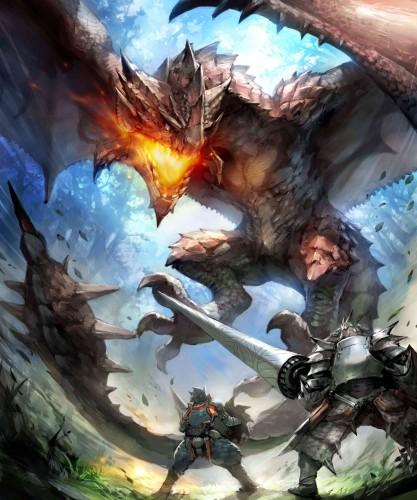
\includegraphics[width=\linewidth]{assets/ext/rathalos-cover.jpg}
\hbSBSep{}%
\textit{Terrible wyverns called "Kings of the Skies". Along with Rathians, they stake wide territories centered around their nests. Rathalos descend on invaders from the sky, attacking with poison claws and breath of fire.}\\*
\noindent
\includegraphics[height=5pt,width=\linewidth]{assets/stat-block-separator}\par
\begin{hbNakedTable}{LYR}
 & \textbf{Item Name} & \textbf{Sale Price}\\
\tableicon{sac-red} & Flame Sac & 240z\\
\tableicon{claw-red} & Rath Wingtalon & 600z\\
\tableicon{shell-red} & Rathalos Carapace & 650z\\
\tableicon{webbing-red} & Rathalos Webbing & 880z\\
\tableicon{carapace-red} & Rath Marrow & 2,100z\\
\tableicon{monster-jewel-red} & Rathalos Ruby & 9,700z\\
\tableicon{mantle-red} & Rathalos Mantle & 15,000z
\end{hbNakedTable}%\par
{\centering\small\tableicon{crown-small}\,1,540\,cm\quad\tableicon{crown-gold}\,2,104\,cm\par}
\end{hbMonsterNote}

\begin{hbMonsterNoteWide}[b]
\begin{multicols}{2}
\begin{hbStatBlock}
\noindent\begin{minipage}[c]{1cm}%

\includegraphics[width=\linewidth]{assets/ext/icons/rathalos.png}%
\end{minipage}\hfill%
\begin{minipage}{\dimexpr -4pt-1cm+\linewidth}%
\subsection*{Rathalos}%
\hbSBType{Huge flying wyvern, unaligned}
\end{minipage}\\*[3pt]
\begin{hbStatBlockDescription}
\item[Armor Class] 16 (natural armor)
\item[Hit Points] 350 (6d10 + 318)
\item[Speed] 25\,ft., fly 60\,ft.
\end{hbStatBlockDescription}
\SBSep
\hbSBAttributes{23}{10}{19}{10}{13}{16}
\SBSep
\begin{hbStatBlockDescription}
\item[Saving Throws] Dex +3, Con +7, Wis +4
\item[Skills] Perception +4
\item[Damage Resistances] fire, poison
\item[Senses] passive Perception 14
\item[Languages] \hbNone
\item[Challenge] 8 (3,900 XP)
\end{hbStatBlockDescription}
\SBSep

\paragraph*{Keen Sight.} Rathalos has advantage on Wisdom (Perception) checks that rely on sight.

\paragraph*{Multiturn.} Rathalos takes two turns each round instead of one. Roll initiative seperately for each one. He may not move more than his Move score each round.

\paragraph*{Rage.} When Rathalos has lost 100 hit points, he becomes enraged. While enraged, he takes three turns instead of two, has disadvantage on Dexterity saving throws and certain special attacks become available to him. At the end of each round, Rathalos must make a DC 15 Constitution saving throw to maintain the rage. When the rage ends, Rathalos takes three levels of exhaustion.

\paragraph*{Poison.} The target must make a DC 13 Constitution saving throw or become poisoned. While poisoned, the target takes 7 (2d6) poison damage at the start of each of its turns. A poisoned creature can repeat the saving throw at the end of each of its turns, ending the effect on itself on a success. While Rathalos is enraged, the poison's save DC increases to 16.

\subsubsection*{Actions}

\paragraph*{Multiattack.} Rathalos makes two bite attacks (or equivalent body parts).

\paragraph*{Bite/Wingtalon/Tail/Slam.} \textit{Melee Weapon Attack:} +8 to hit, reach 10\,ft., one target. Hit: 16 (2d10 + 5) piercing damage.

\paragraph*{Claw.} \textit{Melee Weapon Attack:} +8 to hit, reach 0\,ft., one target. Hit: 14 (2d8 + 5) slashing damage and apply poison.

\paragraph*{Roar.} Rathalos lets out a terrifying roar. Each creature within 120 feet of Rathalos and able to hear him must make a DC 13 Constitution saving throw or be freightened and loose concentration. A frightened creature can repeat the saving throw at the end of each of its turns, ending the effect on itself on a success. When Rathalos first becomes enraged, he may roar as a reaction. While Rathalos is enraged, the roar's save DC increases to 16.

\paragraph*{Wing Reatreat.} Rathalos beats his wings, to gain height or distance. All medium or smaller creatures within 10 feet must succeed at a DC 15 Strength saving throw or be knocked prone and lose their reaction.

\paragraph*{Fire Breath.} All creatures in a 20 foot cone in front of Rathalos must make a DC 15 Dexterity saving throw, taking 28 (8d6) fire damage on a failed save, or half as much damage on a successful one.

\paragraph*{Inferno.} Rathalos bathes an area 20 feet in diameter in flame. Creatures inside this area must make a DC 15 Dexterity saving throw, taking 22 (5d8) fire damage on a failed save, or half as much damage on a successful one. The area remains on fire for 3 rounds (or longer, if there is a lot flammable material, like dry undergrowth). A creature ending its turn in the area takes 22 (5d8) fire damage at the end of each of its turns. A creatures takes the same damage when it enters the area for the first time. Rathalos may only use this action while enraged.

\end{hbStatBlock}
\end{multicols}
\end{hbMonsterNoteWide}

\paragraph*{Not easily provoked, not easily calmed.} Rathalos hunts only by daylight, and will usually fly out to hunt every day. However, due to the size of his territory, he may not be seen every day, though Rathalos is known to have favorite spots that he returns to often. When not out hunting, Rathalos usually sleeps to conserve energy. Unprovoked, he will typically not attack humans unless he feels that his territory is threatened, such as when he spots a large gathering. The main exception is a threat to his roost and especially to his eggs. No creature, human or monster, is allowed close to its roost and will always be attacked and repelled. Nevertheless, there are rumours of large wyvern eggs being traded on the black market by daredevil thrill-seekers\ldots

\paragraph*{Life in the monarchy.} Rathalos will take and hold the spot of top predator in any environment he inhabits, and he is one of the most common large wyverns. As a result, many villages around the world know what it means to live with the red shadow in the sky. Despite this fearsome monarch, the Guild understands that Rathalos has an important place in the ecosystem, and that he is preferable to many of the alternatives, such as \tableicon{glavenusS}~Glavenus and that there have been times where all that stood between a village and a terrible threat was Rathalos, defending his territory. Sometimes, living under a king is not so bad.

% Intended pagebreak here!
\pagebreak[3]

\subsection{Combat Tactics}
For Rathalos, there are two types of fighting: Hunting, and defending territory. For the first, he will make use of his venom claws and not commit to an extended engagement.

When defending his territory, however, he will engage and it will not take long for him to bring his full power to bear, making full use of his weight as well as his fire breath, which he keeps in reserve for such occasions, due to its high energy cost.

Rathalos is an aerial predator and will use his ability to fly frequently in order to gain an advantage. From his high position, he makes swooping strikes, only to take to the air again. While he would engage another trespassing wyvern wherever he discovers it, Rathalos may sometimes hold back for a time before deciding to attack hunter parties, waiting for them to enter unfavorable terrain, such as a narrow ravine. If given the choice, he will prefer places where his enemies cannot effectively escape his fire breath.

\subsection*{Moves}

\paragraph*{Swooping Claws.} Rathalos uses the Wing Retreat, and moves upwards. In the air, he chooses a mark. A successful Wisdom (Animal Handling) check may reveal who is going to be attacked. On his next turn, he swoops down again, using his claw attack to poison the target.

\paragraph*{Into the frying pan.} When Rathalos becomes enraged, he can roar as a reaction. This may cause some enemies to become frightened and run away. It can then use Inferno to cut off their retreat.

\paragraph*{Talon Pin.} Another typical attack after coming out of the air is a pinning claw attack, holding the target down (his grapple counts as being restrained) and tearing into the helpless target. It can be very difficult to escape from this pinning move without help.

\begin{hbNarrowTable}[b]{Carves\hbNone roll 6 times}{RY}
\textbf{d100} & \textbf{Item}\\
01-30 & \tableicon{shell-red} Rathalos Carapace\\
31-55 & \tableicon{claw-red} Rath Wingtalon\\
56-70 & \tableicon{sac-red} Flame Sac x1d4\\
71-84 & \tableicon{webbing-red} Rathalos Webbing\\
85-93 & \tableicon{carapace-red} Rathalos Marrow\\
94-98 & \tableicon{monster-jewel-red} Rathalos Ruby\\
99-00 & \tableicon{mantle-red} Rathalos Mantle
\end{hbNarrowTable}

